\documentclass[11pt, aspectratio=169]{beamer}
% \usefonttheme[onlymath]{serif}
% Autocompletions:
% wit: begin wideitemize
% bit: begin itemize
  % { "trigger": "it", "contents": "\\textit{$1}$0"},
  %               { "trigger": "bf", "contents": "\\textbf{$1}$0"},
  %               { "trigger": "em", "contents": "\\emph{$1}$0"},
  %               { "trigger": "tt", "contents": "\\texttt{$1}$0"},
  %               { "trigger": "un", "contents": "\\underline{$1}$0"},

  %               { "trigger": "bs", "contents": "\\bigskip"},
  %               { "trigger": "ms", "contents": "\\medskip"},
  %               { "trigger": "ss", "contents": "\\smallskip"},

  %               { "trigger": "use", "contents": "\\usepackage"},
        
                % { "trigger": "beq", "contents": "\\[\n$0\n\\]"},               
  %               { "trigger": "beqn", "contents": "\\begin{equation}\n$0\n\\end{equation}\n"},


\usepackage{pgfpages}
% These slides also contain speaker notes. You can print just the slides,
% just the notes, or both, depending on the setting below. Comment out the want
% you want.
\setbeameroption{show notes}
\setbeameroption{hide notes} % Only slide
%\setbeameroption{show only notes} % Only notes
%\setbeameroption{show notes on second screen=right} % Both

% \usepackage{helvet}
% \usepackage[default]{lato}
% \usepackage[T1]{fontenc}

\usepackage{array}

\usepackage{verbatim}
\setbeamertemplate{note page}{\pagecolor{yellow!5}\insertnote}

\usepackage{tikz}
\usetikzlibrary{positioning}
% \usetikzlibrary{snakes}
\usetikzlibrary{decorations}
\usetikzlibrary{calc}
\usetikzlibrary{arrows}
\usetikzlibrary{decorations.markings}
\usetikzlibrary{shapes.misc}
\usetikzlibrary{matrix,shapes,arrows,fit,tikzmark}
\usepackage{amsmath}
\usepackage{mathpazo}
\usepackage{hyperref}
\usepackage{lipsum}
\usepackage{multimedia}
\usepackage{graphicx}
\usepackage{multirow}
\usepackage{graphicx}
\usepackage{dcolumn}
% \usepackage{enumitem}
\usepackage{bbm}
\newcolumntype{d}[0]{D{.}{.}{5}}

\newcommand{\Skip}{\vspace{1em}}
\newcommand{\Squish}{\vspace{-1em}}


\usepackage{changepage}
\usepackage{appendixnumberbeamer}
\newcommand{\beginbackup}{
   \newcounter{framenumbervorappendix}
   \setcounter{framenumbervorappendix}{\value{framenumber}}
   \setbeamertemplate{footline}
   {
     \leavevmode%
     \hline
     box{%
       \begin{beamercolorbox}[wd=\paperwidth,ht=2.25ex,dp=1ex,right]{footlinecolor}%
%         \insertframenumber  \hspace*{2ex} 
       \end{beamercolorbox}}%
     \vskip0pt%
   }
 }
\newcommand{\backupend}{
   \addtocounter{framenumbervorappendix}{-\value{framenumber}}
   \addtocounter{framenumber}{\value{framenumbervorappendix}} 
}


\usepackage{graphicx}
\usepackage[space]{grffile}
\usepackage{booktabs}

% These are my colors -- there are many like them, but these ones are mine.
\definecolor{blue}{RGB}{0,114,178}
\definecolor{red}{RGB}{213,94,0}
\definecolor{yellow}{RGB}{240,228,66}
\definecolor{green}{RGB}{0,158,115}

\hypersetup{
  colorlinks=false,
  linkbordercolor = {white},
  linkcolor = {blue}
}


%% I use a beige off white for my background
\definecolor{MyBackground}{RGB}{255,253,218}

%% Uncomment this if you want to change the background color to something else
%\setbeamercolor{background canvas}{bg=MyBackground}

%% Change the bg color to adjust your transition slide background color!
\newenvironment{transitionframe}{
  \setbeamercolor{background canvas}{bg=yellow}
  \begin{frame}}{
    \end{frame}
}

\setbeamercolor{frametitle}{fg=blue}
\setbeamercolor{title}{fg=black}
\setbeamertemplate{footline}[frame number]
\setbeamertemplate{navigation symbols}{} 
\setbeamertemplate{itemize items}{-}
\setbeamercolor{itemize item}{fg=blue}
\setbeamercolor{itemize subitem}{fg=blue}
\setbeamercolor{enumerate item}{fg=blue}
\setbeamercolor{enumerate subitem}{fg=blue}
\setbeamercolor{button}{bg=MyBackground,fg=blue,}



% If you like road maps, rather than having clutter at the top, have a roadmap show up at the end of each section 
% (and after your introduction)
% Uncomment this is if you want the roadmap!
\AtBeginSection[]
{
   \begin{frame}
       \frametitle{Roadmap of Talk}
       \tableofcontents[currentsection]
   \end{frame}
}
\setbeamercolor{section in toc}{fg=blue}
\setbeamercolor{subsection in toc}{fg=red}
\setbeamersize{text margin left=1em,text margin right=1em} 

\newenvironment{wideitemize}{\itemize\addtolength{\itemsep}{10pt}}{\enditemize}
\newenvironment{wideenumerate}{\enumerate\addtolength{\itemsep}{10pt}}{\endenumerate}
\newenvironment{widedescription}{\description\addtolength{\itemsep}{10pt}}{\enddescription}






\title[]{\textcolor{blue}{Estimating Production Functions}}

\author[CM]{Charlie Murry}
% \institute{Boston College}

% \author[PGP]{}
% \institute[FRBNY]{\small{\begin{tabular}{c c c}
% Author A &&  Paul Goldsmith-Pinkham  \\
% Somewhere Fancy && FRBNY \\ \\

% Author C && Author D   \\
% \multicolumn{3}{c}{Somewhere Fancy} \\
% \end{tabular}}}

% \date{\today}


\begin{document}

%%% TIKZ STUFF
\tikzset{   
        every picture/.style={remember picture,baseline},
        every node/.style={anchor=base,align=center,outer sep=1.5pt},
        every path/.style={thick},
        }
\newcommand\marktopleft[1]{%
    \tikz[overlay,remember picture] 
        \node (marker-#1-a) at (-.3em,.3em) {};%
}
\newcommand\markbottomright[2]{%
    \tikz[overlay,remember picture] 
        \node (marker-#1-b) at (0em,0em) {};%
}
\tikzstyle{every picture}+=[remember picture] 
\tikzstyle{mybox} =[draw=black, very thick, rectangle, inner sep=10pt, inner ysep=20pt]
\tikzstyle{fancytitle} =[draw=black,fill=red, text=white]
%%%% END TIKZ STUFF

% Title Slide (will go at the bottom of title slide)
\begin{frame}
\maketitle
  % \centering The views expressed do not necessarily reflect the position of the Federal Reserve Bank of New York or the Federal Reserve System.
\end{frame}

% INTRO
% \section[intro]{Introduction} % (fold)
% \label{sec:introduction}

\begin{frame}{Motivation\footnote{I borrow from a variety of sources including Victor A's handbook chapter and Paul Grieco's and Peter Newberry's notes from Penn State and Paul Scott's notes from NYU.}}

\emph{The production function is an object of primary economic interest.}

\Skip
\begin{wideitemize}
	\item Characterize firm's cost function.
	\item What are returns to scale in an industry? 
	\item How persistent is productivity?
	\item Do input elasticities change over time?
	\item What is the impact of new technology?
	\item What is impact of trade/macro policies on production?
	\item Is productivity correlated with exporting, importing, etc?
\end{wideitemize}

% \begin{columns}[T] % align columns
% \begin{column}{.58\textwidth}
%   \begin{wideitemize}
%     \item This slide deck has suggestions and ideas for a better presentation
%     \item The goal is minimalist design, but that doesn't mean boring slides
%     \item Making slides is hard work - the goal is to make default set
%       of slides that look nicer and encourage better design
%     \item Read \emph{\textcolor{blue}{\href{https://www.amazon.com/Better-Presentations-Guide-Scholars-Researchers/dp/0231175213/}{Jon Schwabish's ``Better Presentations''}}}
%   \end{wideitemize}
% \end{column}%
% \hfill%
% \begin{column}{.38\textwidth}
%   \makebox[\linewidth][c]{
%     \resizebox{\linewidth}{!}{
%       \includegraphics{how-to-draw-an-owl.pdf}
%     }
%   }
% \end{column}%
% \end{columns}
\end{frame}


\begin{frame}[c]\frametitle{More questions...}

\begin{wideitemize}
	\item What contributes to economic growth?
	\item Role of skill-biased tech change. 
	\item Learning-by-doing?
	\item Do more productive firms choose higher quality or charge higher markups?
\end{wideitemize}
    


\end{frame}


\begin{frame}[c]\frametitle{Fix Ideas}
   
\begin{equation}\label{eq:CobbDouglas}
	Y_{it} = L_{it}^{\beta_{\ell}}K_{it}^{\beta_k}U_{it}
\end{equation}


\Skip
\begin{wideitemize}
	\item $U$ -- (total factor) productivity.
	\begin{itemize}
		\item in contrast to labor productivity: $Y/L$
	\end{itemize}
	\item $L,K$ -- input choices of firms.	
	\item $\beta$ -- output elasticities.
\end{wideitemize}

\bigskip
\textbf{Goal:} Estimate $\beta$.

\bigskip
\textbf{The catch:} Choice of $L$ a function of $U$.
\end{frame}

\begin{frame}[c]\frametitle{Fix Ideas -- Data}

\textbf{Typical dataset:}
\begin{wideitemize}
	\item Yearly (typically) data.
	\item Measure of output: quantity, revenues, value-added (R minus cost of materials)
	\item Inputs: laborers, capital stock, investment, R\&D, materials, energy costs. 
	\item USA: Compustat, US Census Long. Research Database.
	\item Europe: Panel data from central banks. 
	\item Other: Chile, Columbia, France, Estonia, etc.
\end{wideitemize}


\end{frame}


\begin{frame}[c]\frametitle{Framework: Production by Firms/plants}

\begin{wideitemize}
	\item Production is dynamic by its nature. 
	\item Why? Capital (K) requires investment (I) and depreciates. 
	\item Firms engage in other activities that are state variables.
	\begin{itemize}
	 	\item R\&D
	 	\item Entry/exit 
	 	\item entry into new/export markets
	 \end{itemize} 
	 \item Unlike in demand estimation, it will be harder to ignore this for estimation because dynamics are at the core of even the baseline model.
	 \item Models of industry dynamics rely on heterogeneous (and stochastic) productivity.
	 \begin{itemize}
	 	\item Jovanovic (1982), Hopanhyan (1992), Melitz (2003)
	 \end{itemize}
\end{wideitemize}
    
\end{frame}


\begin{frame}[c]\frametitle{Econometric Simultaneity}
    
Take logs of Eq \ref{eq:CobbDouglas}:

\begin{equation}
	y_{it} = \beta_{\ell} \ell_{it} + \beta_k k_{it} + \omega_{it} + \varepsilon_{it}    	
\end{equation}    

\begin{wideitemize}
	\item $\varepsilon$ is just random and not known at the time of choosing $K$ and $L$. 
	\item $\omega_{it}$ is productivity, known to the firm.
	\item $\ell_t$ or $k_t$ could be chosen with knowledge of $\omega_t$
	\item Typically we think that $k$ is chosen at $t-1$ (as investment, $i_{t-1}$)
	\item But more productive firms should choose more $\ell$.
\end{wideitemize}

\end{frame}

\begin{frame}[c]\frametitle{Classic solutions to the simultaneity problem}
    
\textbf{Input prices (or other variables) as instruments:}
\begin{wideitemize}
	\item Sometimes data not available.
	\item Almost never any variation in data across firms. 
	\item Even if this exists, the variation is probably not exogenous. 
\end{wideitemize}

\bigskip
\textbf{Fixed Effects:}
\begin{wideitemize}
	\item Assumption: $\omega_{it}$ is really $\omega_{i} (+\varepsilon_{it})$
	\item Probably not suitable for long panels. 
	\item Assumes no change in firm-specific technology -- this rules out some interesting questions from the beginning. 
	\item Differencing kills variation in $k$.
\end{wideitemize}

\end{frame}


\begin{frame}[c]\frametitle{Classic solutions to the simultaneity problem}
    
\textbf{Dynamic Panel Methods}
\begin{wideitemize}
	\item See Arellano and Bond (1991).
	\item Let's put some structure on TFP. 
	\item $\omega_t = \rho \omega_{t-1} + \xi_t$
	\item See problem set...
\end{wideitemize}


\end{frame}


\begin{frame}[c]\frametitle{Econometric Selection}
    
% wit    
\begin{wideitemize}
	\item Firms that exit have low productivity draws. 
	\begin{wideitemize}
		\item See Hopanhyan (1992) or Melitz (1993).
	\end{wideitemize}	
	\item Or, variable like ``export status'' will be endogenous, as more productive firms may be more willing to export/import.
	\item We will basically punt on this for now, but it is discussed at length in OP. 
\end{wideitemize}

\end{frame}


\begin{frame}[c]\frametitle{Biased Estimates}

\textbf{Simultaneity}
\begin{wideitemize}
	\item Upward bias in labor coefficient.
	\item More efficient firms choose more labor. 
\end{wideitemize}

\bigskip
\textbf{Selection}
\begin{wideitemize}
	\item Downward bias in capital coefficient.
	\item Firms with high capital have very low $\omega$ cutoffs for exit. 
	\item exit distorts the joint dist. of $k$ and $\omega$.
	\item \emph{Conditional on firm surviving}, there is negative correlation between $k$ and $\omega$, although in reality we expect low $\omega$ firms to be low $k$ firms.
\end{wideitemize}

    


\end{frame}


% section introduction (end)

\section[OP]{Olley and Pakes} % (fold)
\label{sec:olley_and_pakes}


\begin{frame}[c]\frametitle{Olley and Pakes (1996)}
    

Propose alternative solution to simultaneity (and selection) problem.

\bigskip
\textbf{Idea}

\begin{wideitemize}
	\item Greater (optimal) investment this period implies the firm realized a higher $\omega_t$.
	\item Use investment ($i_t$) to ``proxy'' for TFP ($\omega_t$).
	\begin{wideitemize}
		\item Remember: investment does not get used until next period!
	\end{wideitemize}
	\item This only works under certain conditions -- \emph{which is the innovation in this paper.} 
\end{wideitemize}

\end{frame}


\begin{frame}[c]\frametitle{OP - Details\footnote{The description here follows ACF.}}
    
\textbf{OP1: Information}\\
% \begin{wideitemize}
Firm info set ($\mathcal{I}_t$) includes only current and past $\omega$. $\varepsilon$ is exogenous: $E[\varepsilon_t \mid \mathcal{I}_t] = 0$. 
% \end{wideitemize}

\bigskip
\textbf{OP2: First Order Markov}\\
$p(\omega_{i,t+1} \mid \mathcal{I}_{it}) = p(\omega_{i,t+1} \mid \omega_{it}) $

\bigskip
\textbf{OP3: Timing}\\
Firms accumulate capital according to $k_{it} = \kappa(k_{i,t-1},i_{i,t-1})$. Labor is not dynamic. 

\bigskip
\textbf{OP4: Scalar Unobservable}\\
Firms investment decisions: $i_{it} = f_t(k_{it},\omega_{it})$.

\bigskip
\textbf{OP5: Strict Monotonicity}\\
$f_t(k_{it},\omega_{it})$is strictly increasing in $\omega_{it}$.

\end{frame}



\begin{frame}[c]\frametitle{Investment as a Proxy}
    
\textbf{OP2: First Order Markov}\\
$p(\omega_{i,t+1} \mid I_{it}) = p(\omega_{i,t+1} \mid \omega_{it}) $

\bigskip
\textbf{OP5: Strict Monotonicity}\\
$f_t(k_{it},\omega_{it})$is strictly increasing in $\omega_{it}$.

\bigskip
These together imply: firms with higher $\omega_{it}$ have higher expected marginal product of capital in the future and will invest more. 

\bigskip
As ACF point out, proving this is tedious and may not extend to all models, but is general enough for relatively straightforward models with C-D or trans-log PFs.

\begin{wideitemize}
 	\item Involves analyzing the specific dynamic programming problem.
\end{wideitemize}



\end{frame}


\begin{frame}[c]\frametitle{Econometric Procedure -- First Stage}
    
\begin{wideitemize}
	\item Invert investment policy function: 
	$$\omega_{it} = h(k_{it},i_{it})$$
	(remember we can do this because $i$ is monotonic in $\omega$!)
	\item Then plug in for $\omega$ in the linear (in logs) production function:
	$$	y_{it} = \beta_{\ell} \ell_{it} + \beta_k k_{it} + h(k_{it},i_{it}) + \varepsilon_{it},$$
	or
	$$	y_{it} = \beta_{\ell} \ell_{it} + \Phi_t(k_{it},i_{it}) + \varepsilon_{it}.$$
	% $$\Phi_t(k_{it},i_{it}) = \beta k_{it} + h(k_{it},i_{it}).$$
	\item \footnotesize(pause here and think about what is going on...)
\end{wideitemize}

\end{frame}


\begin{frame}[c]\frametitle{Econometric Procedure -- First Stage}
    
\begin{wideitemize}
	\item First stage regression:
	$$	y_{it} = \beta_{\ell} \ell_{it} + \Phi_t(k_{it},i_{it}) + \varepsilon_{it},$$
	and recall
	$$\Phi_t(k_{it},i_{it}) = \beta_k k_{it} + h(k_{it},i_{it}).$$
	\item Notice that $k$ enters multiple places, and $h()$ is unknown, so the only primitive we can recover is $\beta_{\ell}$. 
	\item But we can also recover $\hat{\Phi}(k_{it},i_{it})$ -- treat this non-parametrically.
\end{wideitemize}

\end{frame}


\begin{frame}[c]\frametitle{Econometric Procedure -- Second Stage}
    
\begin{wideitemize}
	\item We have $\hat{\Phi}(k_{it},i_{it})$ and $\hat{\beta}_{\ell} \ell_{it}$ in hand from the first stage. 
	\item Decompose $\omega$ into the expected part (given the state $\mathcal{I}$) plus an innovation: 
	$$\omega_{it} = E[\omega_{it}\mid\mathcal{I}_{it}] + \xi_{it} = E[\omega_{it}\mid\omega_{i,t-1}] + \xi_{it} = g(\omega_{i,t-1}) + \xi_{it}$$
	\item Now plug this into the production function:
	$$y_{it} = \beta_{\ell} \ell_{it} + \beta_k k_{it} + g(\Phi_{t-1}(k_{i,t-1},i_{i,t-1})-\beta_k k_{i,t-1}) + \xi_{it} + \varepsilon_{it}$$

\end{wideitemize}


\end{frame}


\begin{frame}[c]\frametitle{Econometric Procedure -- Second Stage}
    
\begin{wideitemize}
	\item Use the following moment:
	$$E[\xi_{it} + \varepsilon_{it} \mid \mathcal{I}_{it}] = 0$$
	or 
	$$E[y_{it} - \beta_{\ell} \ell_{it} - \beta_k k_{it} - g(\Phi_{t-1}(k_{i,t-1},i_{i,t-1})-\beta k_{i,t-1}) \mid \mathcal{I}_{it}] = 0.$$
\end{wideitemize}

\bigskip
\textbf{Procedure}\footnote{if $g$ is linear then you could use OLS.}

\begin{enumerate}
	\item plug-in first-stage estimates: $\hat{\beta_{\ell}}$ and $\hat{\Phi}$ and pick parametric form for $g()$.
	\item guess $\beta_k$.
	\item Estimate $g()$: 
	$$ \Phi_{it} = \beta_k k_{it} + \underbrace{g(\Phi_{i,t-1} - \beta_k k_{i,t-1})}_{E[\omega_t \mid \mathcal{I}_t]} + \xi_{it}$$
	\item Back out $\hat{\xi}(\beta_k)$
	\item Evaluate $E[\xi|\mathcal{I}]$
	\item go back to 2. until $E[\xi|\mathcal{I}]=0$.
\end{enumerate}

\end{frame}



\begin{frame}[c]\frametitle{OP Results}
    
\centering
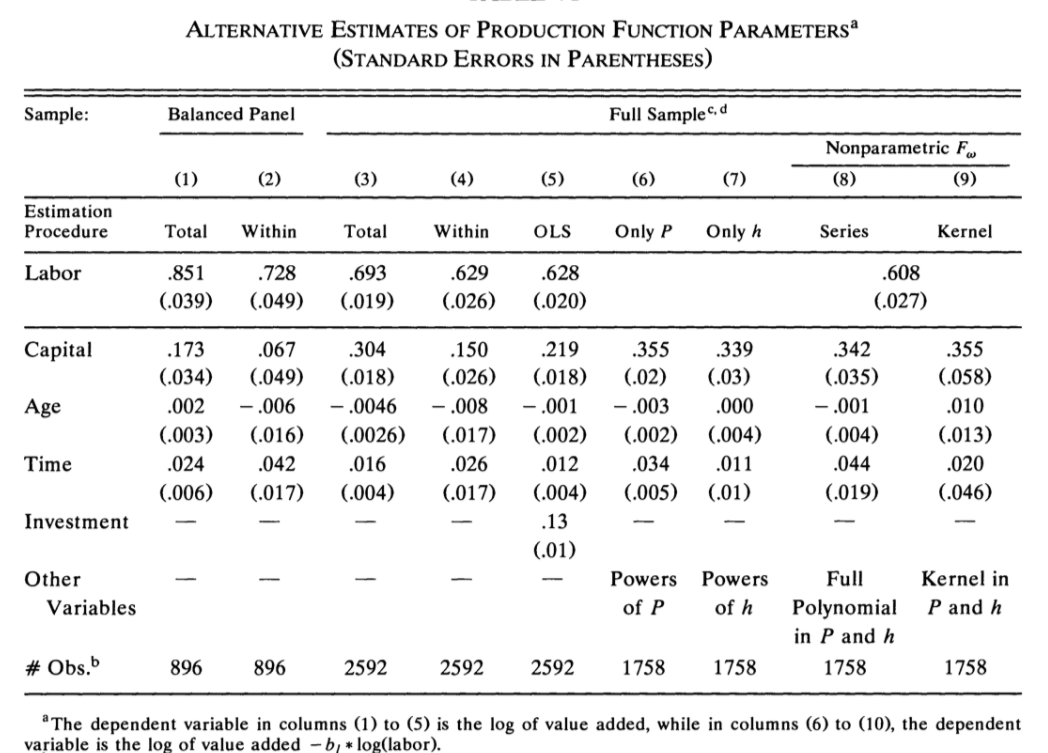
\includegraphics[height=0.9\textheight]{OPTable6.png}


\end{frame}


\begin{frame}[c]\frametitle{Application}
    

\begin{wideitemize}
	\item How does productivity change of telecom equipment manufacturers after massive deregulation in telecom industry? [1977 and 1984]
	\item Productivity:
	$$p_{it} = exp(y_{it} - \hat{\beta}_{\ell}\ell_{it} - \hat{\beta}_{k}k_{it} )$$
\end{wideitemize}

\centering
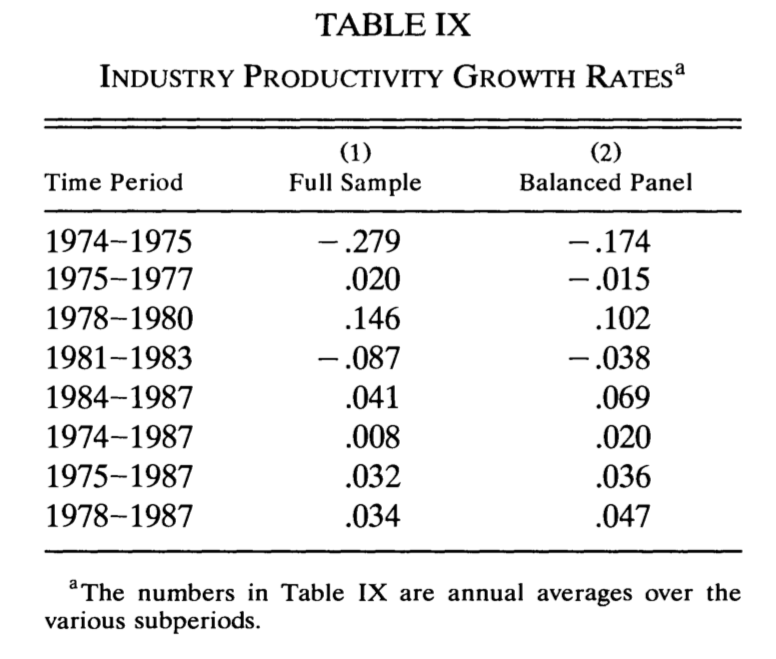
\includegraphics[scale=.2]{OP-Table9.png}

\end{frame}



% section olley_and_pakes (end)

\section[LP]{Levinsohn and Petrin} % (fold)
\label{sec:levinsohn_and_petrin}

\begin{frame}[c]\frametitle{Levinsohn and Petrin (2003)}
    
    \textbf{Key Insight}

    \begin{wideitemize}
    	\item Use materials instead of investment to proxy for TFP.
    	\item Today's choice of intermediate inputs is correlated with today's productivity.
    \end{wideitemize}
    
    \bigskip
    \textbf{Why?}
    \begin{wideitemize}
    	\item Investment proxy not valid for plants with zero investment.
    	\item Literature has shown investment is ``lumpy''.
    	\begin{wideitemize}
    		\item May not immediate respond to productivity shocks.
    		\item Potential adjustment issues or measurement issues.
    	\end{wideitemize}
    	
    \end{wideitemize}
    
\end{frame}



\begin{frame}[c]\frametitle{Investment Zeros}

\centering    
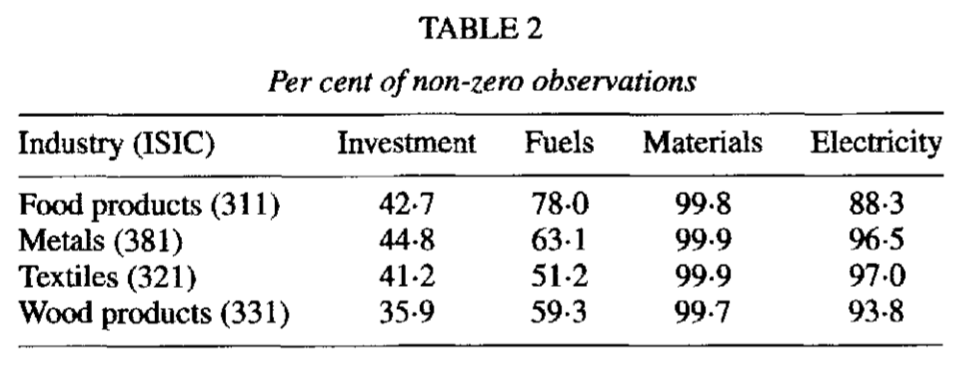
\includegraphics[height=.5\textheight]{LP-Table2.png}

\end{frame}




\begin{frame}[c]\frametitle{LP Estimation}
    
\begin{wideitemize}
	\item First Stage:
	$$	y_{it} = \beta_{\ell} \ell_{it} + \Phi_t(k_{it},m_{it}) + \varepsilon_{it}$$
	\item Estimate $\hat{\beta}_{\ell}$ and $\hat{\Phi}()$ treating $\Phi$ non-parametrically.
	\item Second Stage:	
	$$E[\xi_{it} + \varepsilon_{it} \mid \mathcal{I}_{it}] = 0$$
	or 
	\begin{align*}
	E[y_{it} - \beta_{\ell} \ell_{it} - \beta_k k_{it} - \beta_m m_{it} -& \\
	g(\Phi_{t-1}(k_{i,t-1},m_{i,t-1})-&\beta_k k_{i,t-1} - \beta_m m_{i,t-1}) \mid \mathcal{I}_{it}] = 0.
	\end{align*}
\end{wideitemize}

\end{frame}

\begin{frame}[c]\frametitle{Discussion}
    
\begin{wideenumerate}
	\item We need a similar condition on the ``materials'' function as we had on the ``investment'' function in OP: $m(k,\omega)$ is monotonically increasing in productivity ($\omega$).
	\begin{wideitemize}
		\item This relies on properties of the production function.
		\item In OP it also relied this relied on the Markov Perfect Eqm assumption. Note here.
		\item Why? materials is a static input.
	\end{wideitemize}
	\item OP rules out firm specific unobservables affecting investment demand -- firm-specific adjustment costs, prices, etc. 
	\begin{wideitemize}
		\item Why? The scalar unobservable assumption. 
		\item LP can allow for this because $m$ is static, so $m(k_t,\omega_t)$ does not depend on investment. 	
	\end{wideitemize}
	\item In the second stage the need to identify two parameters so they use two moments: 
	$$E[\xi_t \times
	\begin{pmatrix}
	k_t \\
	m_{t-1}
	\end{pmatrix}
	]=0$$
\end{wideenumerate}

\end{frame}



\begin{frame}[c]\frametitle{Results}

\centering    
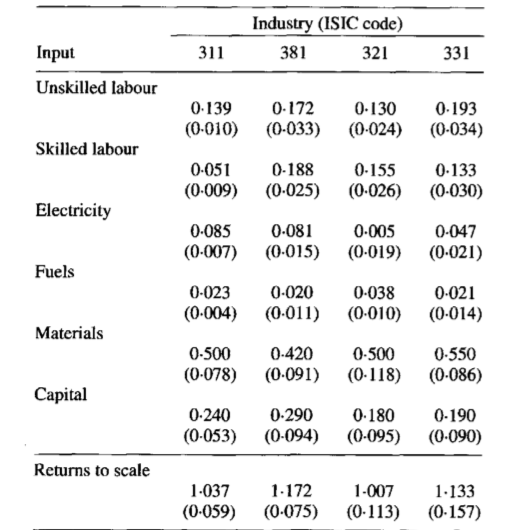
\includegraphics[height=.95\textheight]{LP-Table3.png}

\end{frame}


\begin{frame}[c]\frametitle{Results}

\centering    
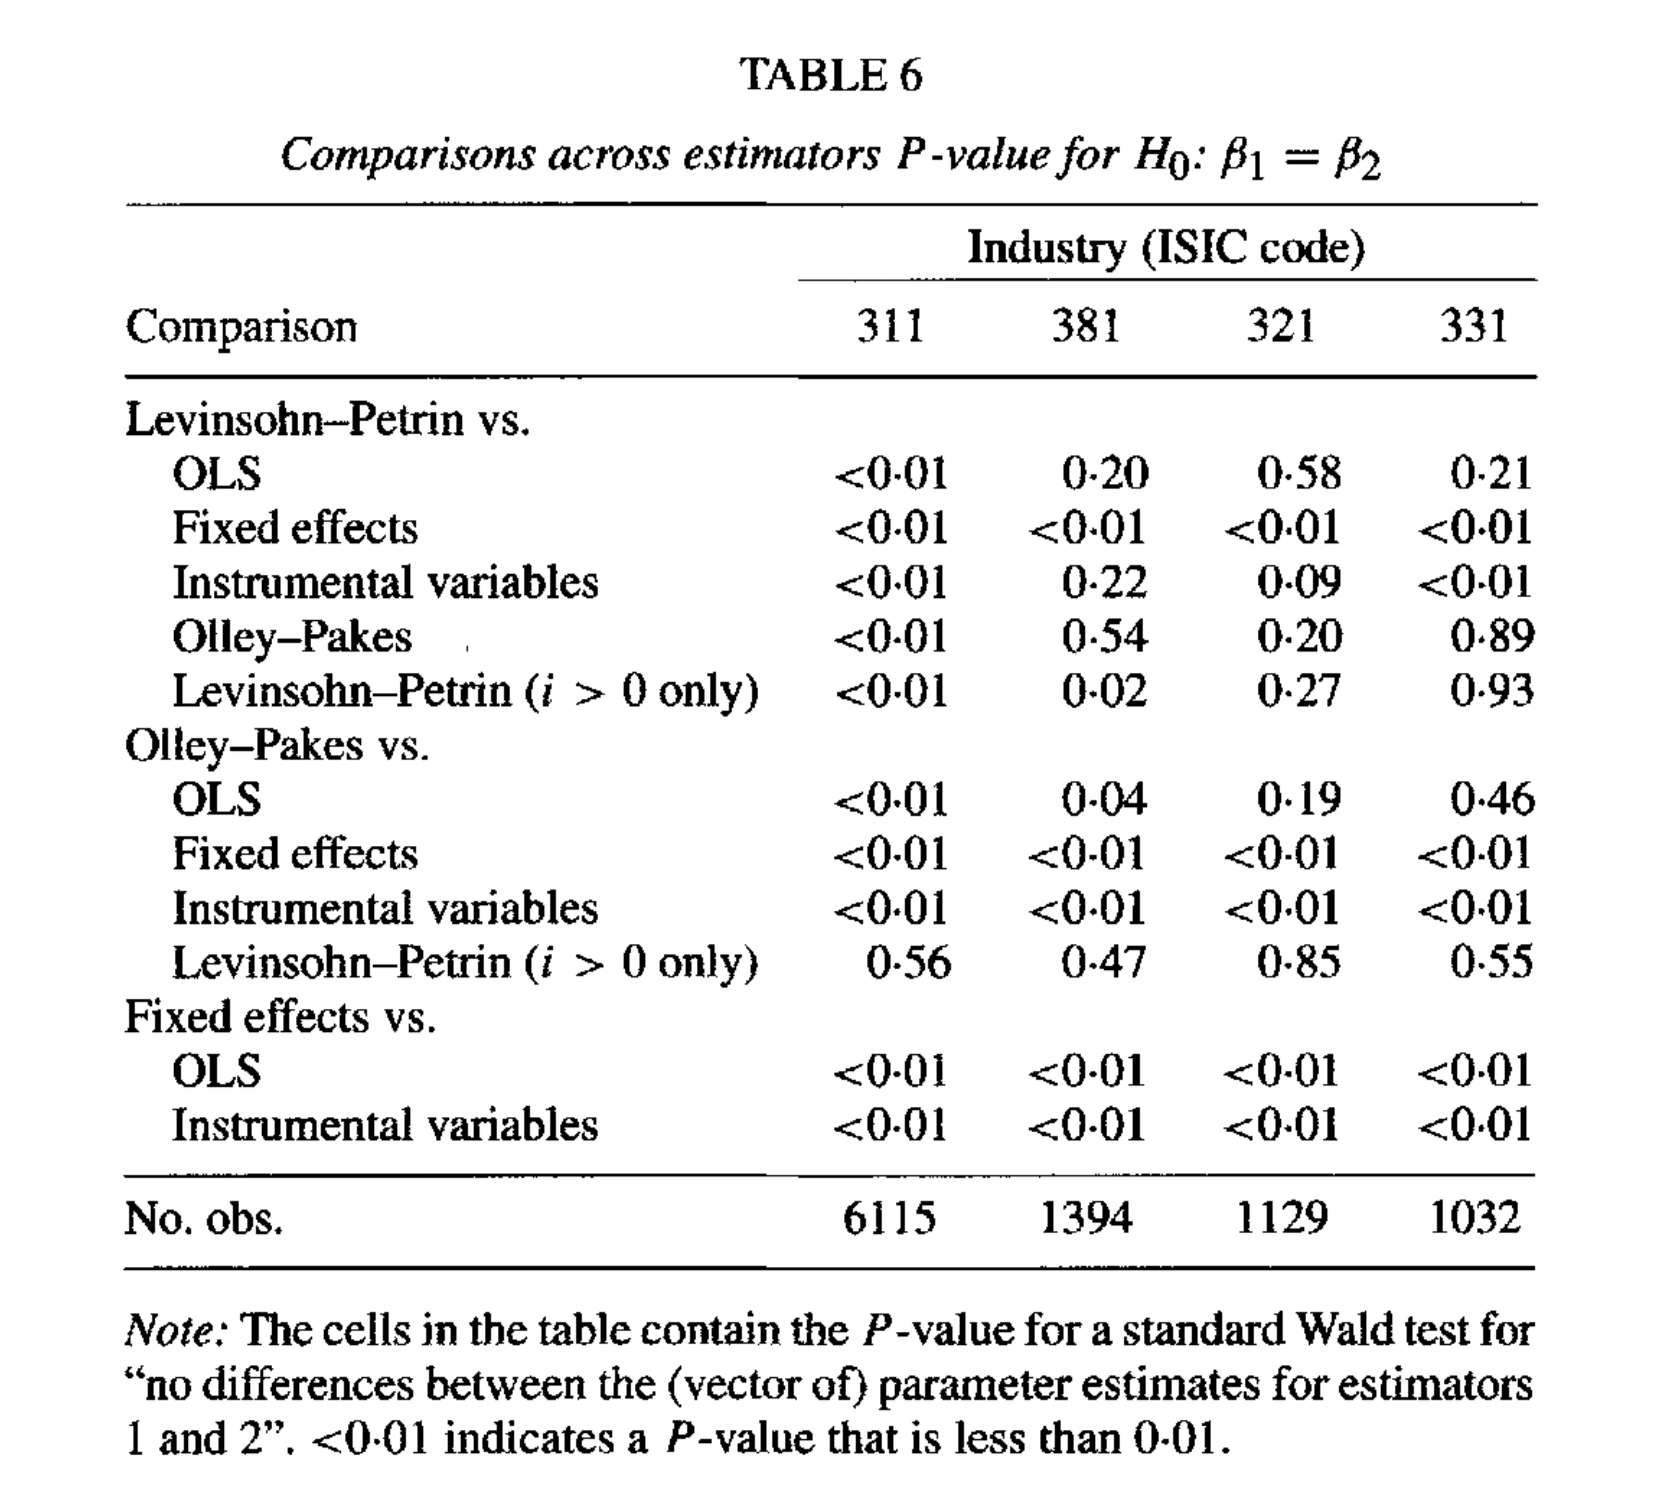
\includegraphics[height=.95\textheight]{LP-Table6.png}

\end{frame}


% section levinsohn_and_petrin (end)


\section[ACF]{Ackerberg, Caves, and Frazer} % (fold)
\label{sec:ackerberg_caves_and_frazer}


\begin{frame}[c]\frametitle{Summary}
    
\textbf{Olley Pakes}\\

Use investment to proxy for unobserved productivity, $\omega$.\\

ALternatives would be: IV, fixed effects, dynamic panel methods.





\Skip
\textbf{Levinsohn and Petrin}\\

Use materials instead. 
\begin{itemize}
	\item No zeros, unlike investment.
	\item weaker assumptions.  
\end{itemize}



\end{frame}


\begin{frame}[c]\frametitle{Ackerberg, Caves, and Frazer (2015)}
    
Conceptual issue with OP/LP: \textbf{functional dependence}.
\begin{wideitemize}
    \item Conditional on $k$, $\omega$ (and $m$), labor is completely determined...oops.
\end{wideitemize}
        
\textbf{Example}        
\begin{wideitemize}
	\item FOC for $m$ is:
	$$\beta_m K_{it}^{\beta_k}L_{it}^{\beta_{\ell}}M_{it}^{\beta_m-1}e^{\omega_{it}} = \frac{p_m}{p_y}$$
	\item then solve for $\omega$ and plug this into the production function:
	$$y_{it} = ln(\frac{1}{\beta_m}) + ln(\frac{p_m}{p_y}) + m_{it} + \varepsilon_{it}$$
	\item But there is no $\beta_{\ell}$ in this equation! So a moment condition based on $\varepsilon$ will not have any co-variation in the data to inform about $\beta_{\ell}$
\end{wideitemize}


\end{frame}


\begin{frame}[c]\frametitle{Functional Dependence}

The point is more general than the example above. 
\begin{wideitemize}
	\item In general, if $\ell$ is \emph{only} a function of $k$, $m$, and $t$, then $\beta_{\ell}$ will not be identified (see Robinsin 1988 for a discussion of partially linear models). 
\end{wideitemize}

\bigskip
What to do? \emph{ACF essentially propose modelling their way out of this issue.}

\Skip
In other words: what assumptions should we have made on the DGP in order for our regressions to make sense.
\begin{wideitemize}
	\item Think about data generating process for $\ell$ that is realistic and implies $\ell$ is not completely pinned down by $\{k,m,t\}$.
	\item ACF consider timing assumptions on the shocks and the choice of $\ell$.
	\item Solution? Assume ``optimization error'' in $\ell$.
	\begin{wideitemize}
		\item Note: ``Optimization error ''in other vars (ie $m$) means we cannot invert $\omega(k,m)$.
		\item In fact, measurement error in general causes problems in this literature. 
	\end{wideitemize}
	
\end{wideitemize}


\end{frame}


\begin{frame}[c]\frametitle{ACF's Alternative DGP}
    
\begin{wideitemize}
	\item Assume $\ell$ set at time $t$
	\item $m$ set at time $t-b$ with $0<b<1$ -- so like a half period.
	$$y_{it} = \beta_{\ell} \ell_{it} + \beta_m m_{it} + \beta_k k_{it} + \omega_{i,t-b} + \eta_{it}$$
	with 
	$$p(\omega_{t-b}\mid \mathcal{I}_{t-1}) = p(\omega_{t-b}\mid\omega_{t-1})$$
	\item there is an unobserved i.i.d. shock to $\ell$ after materials are chosen and before $\ell$ is chosen. 
	\item $\ell$ now has its own shock and it is not a state variable. 
	\item This works, but playing with timing like this can get a bit absurd. 
\end{wideitemize}
    

\end{frame}



\begin{frame}[c]\frametitle{ACF Procedure}
    
\begin{wideitemize}
	\item Consider a value added production function:
	$$y_{it} = \beta_{\ell} \ell_{it} + \beta_k k_{it} + \omega_{i,t-b} + \eta_{it}$$
	with 
	$$k_{it} = \kappa(k_{i,t-1},i_{i,t-1})$$
	\item investment is chosen in $t-1$ and labor ($\ell$) is potentially dynamic -- it can be chosen $t$, $t-1$, $t-b$.
	\item Input demand $m_{it} = \tilde{f_t}(k_t,\ell_t,\omega_t)$ is monotonic in $\omega$.
	\item demand for $m$ is \emph{conditional} on $\ell\,\,$! This is different (and more general).
\end{wideitemize}

\end{frame}

\begin{frame}[c]\frametitle{ACF Procedure -- First Stage}
    
\begin{wideitemize}
	\item In first stage, just recover expected output:
	$$y_{it} = \Phi_t(m_t,\ell_t,k_t) + \varepsilon_{it}$$
	where
	$$\Phi_t(m_t,\ell_t,k_t) =  \beta_{\ell} \ell_{it} + \beta_k k_{it} + \tilde{f_t}(k_t,\ell_t,\omega_t)  $$
	\item Now we can predict productivity:
	$$\omega_{it} = \hat{\Phi}_t - \beta_{\ell} \ell_{it} - \beta_k k_{it} $$
\end{wideitemize}


\end{frame}


\begin{frame}[c]\frametitle{ACF Procedure -- Second Stage}
    

\begin{wideitemize}
	\item Non-parameterically regress $\hat{\omega}_{it}(\beta_{\ell},\beta_k)$ on $\hat{\omega}_{it-1}(\beta_{\ell},\beta_k)$ to get the ``innovations'' to productivity (just like LP). 
	$$\xi_{it} = \hat{\omega}_{it}(\beta_{\ell},\beta_k) - E[\hat{\omega}_{it}(\beta_{\ell},\beta_k) \mid \hat{\omega}_{it-1}(\beta_{\ell},\beta_k)]$$
	\item Estimation using the following moments:
	$$\frac{1}{T}\frac{1}{N}\sum_t\sum_i \hat{\xi} 
	\begin{pmatrix}
		k_{it}\\
		\ell_{i,t-1}
	\end{pmatrix}$$
	\item Intuition? If $\ell$ is chosen after $t-1$ then $\ell_t$ will be correlated with $\xi_t$, then:
	\begin{wideitemize}
		\item $\ell_{t-1}$ is chosen without knowledge of $\xi$ (the innovation),
		\item Certainly $k_{t}$ chosen without knowledge of $\xi$ ($i_{t}$).
	\end{wideitemize}
\end{wideitemize}

\end{frame}




\begin{frame}[c]\frametitle{Discussion}
    
\textbf{Estimation Procedure}    
\begin{wideitemize}
	\item The fact that this is a procedure for a ``value added'' production function is important. 
	\begin{wideitemize}
		\item Gross output pf is Leontief in materials.
		\item Existence of ``value added'' pf is not trivial per se, and there is a (macro) literature that discusses this.
		\item GNR (2018) show that gross output pfs are not identified without additional assumptions!
	\end{wideitemize}
	\item Timing assumption on $\ell$ but this does not conflict with $m$. 
	\begin{wideitemize}
		\item $\ell$ can be (but not need be) chosen
	\end{wideitemize}
	\item Do not estimate $\beta_{\ell}$ in first stage, so functional dependence issue is gone. 
\end{wideitemize}

\end{frame}


\begin{frame}[c]\frametitle{Discussion}
    

\bigskip
\textbf{Measurement}
\begin{wideitemize}
	\item Ideal data is when we have \emph{units} for each variable. (why?)
	\item Generally this is not true for output or inputs other than $L$.
	\begin{wideitemize}
		\item Monetary units of inputs/output are not comparable.
		\item If prices are observed (not common), then we can get back to units, and also use prices as instruments (if exogenous).
	\end{wideitemize}
	\item Firms face downward sloping output demand curves (or up-sloping input supply)?
	\begin{wideitemize}
			\item If every firm does not face the exact same demand, then investment functions will be different, OP/LP not valid. 
			\item Some recent advances along this point --  Klette and Griliches (1996), De Loecker (2011). 
	\end{wideitemize}			
	\item Basically, from the very start (data and measurement), there are a lot of assumptions baked into the standard (OP/LP) techniques.
\end{wideitemize}

\end{frame}

\begin{frame}[c]\frametitle{}
\centering
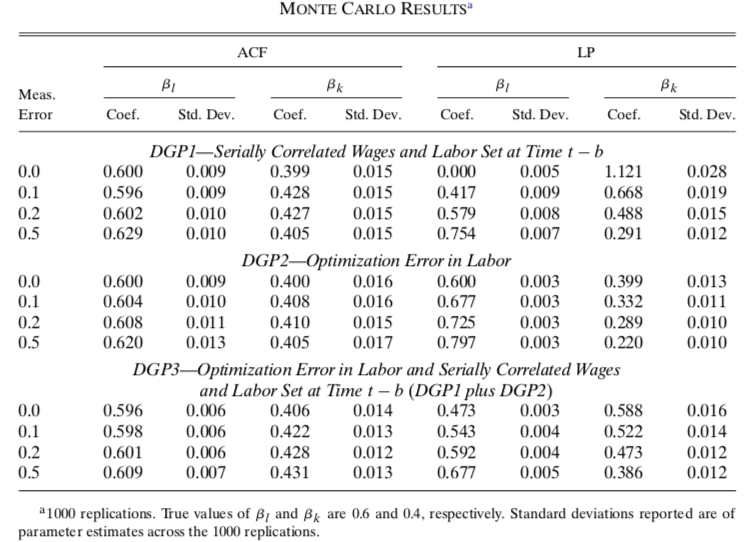
\includegraphics[scale=.42]{ACF - Table1.png}

\end{frame}


\begin{frame}[c]\frametitle{Monte Carlo Description}
    

\begin{wideitemize}
	\item DGP1: Firms face different wages and choose wage at $t-0.5$.
	\begin{wideitemize}
		\item Favorable to ACF. Inconsistent with LP.
	\end{wideitemize}
	\item DGP2: Optimization in $\ell$. And data on $m$ is planned materials.
	\begin{wideitemize}
		\item Consistent with LP, although timing a bit ad hoc.
	\end{wideitemize}	
	\item DGP3: DGP1 + DGP2
	\begin{wideitemize}
		\item Inconsistent with ACF and LP.
	\end{wideitemize}	
\end{wideitemize}

\end{frame}


% section ackerberg_caves_and_frazer (end)


\section{Markups: De Loecker and Warzynski (2012)} % (fold)
\label{sec:de_loecker_and_warzynski_}

\begin{frame}[c]\frametitle{De Loecker and Warzynski (2012)}
    
\begin{wideitemize}
	\item Derive expression for markups ($\mu = P/MC$) from cost minimization of firm.
	\item This expression a function output elasticity. (ding ding!)
	\item We can use our new-found ability to estimate production functions to estimate markups. 
\end{wideitemize}

\end{frame}


\begin{frame}[c]\frametitle{Main Idea}
    
\textbf{Assumption:} variable inputs are set each period to minimize costs. 

\bigskip
\begin{wideitemize}
	\item Cost minimization Lagrangian:
	$$\mathcal{L}(X^1_{it},X^2_{it},K_{it},\lambda_{it}) = \sum_{v=1}^V P^v_{it} X^v_{it} + r_{it}K_{it} + \lambda_{it}(Q_{it} - Q_{t}(\cdot_{it})) $$
	\item where $X^v$ is a flexible input, $P^v$ input prices.\pause
	\item FOC:
	$$ P^v_{it} = \lambda_{it}\frac{\partial Q_t()}{\partial X^v_{it} } $$
	\item Notice that $\lambda$ is the shadow cost of the $Q$ constraint binding, i.e. the marginal cost of production. 
\end{wideitemize}

\end{frame}


\begin{frame}[t]\frametitle{Deriving Markup Expression}
    

\begin{wideitemize}
	\item Multiply by $X^v/Q$:
	$$ \frac{\partial Q_t()}{\partial X^v_{it}} \frac{X^v_{it}}{Q_{it}} 
	= \frac{1}{\lambda} \frac{P^v_{it} X^v_{it}}{Q_{it}}$$\pause
	\item Multiply and divide by output price, $P_{it}$:
	$$ \underbrace{\frac{\partial Q_t()}{\partial X^v_{it}} \frac{X^v_{it}}{Q_{it}}}_{output\,\,elas.} 
	= \mu_{it} \underbrace{\frac{P^v_{it} X^v_{it}}{P_{it}Q_{it}}}_{rev.\,\,share}$$
	\item or markup is a ratio of output elas. to revenue share,
	$$ \mu_{it} = \theta^v_{it} / \alpha^v_{it} $$.
\end{wideitemize}

\end{frame}


\begin{frame}[c]\frametitle{Markup Expression Discussion}
    
	$$ \mu_{it} = \theta^v_{it} / \alpha^v_{it} $$.
\begin{wideitemize}
	\item This actually dates back to at Hall (1988) who computes industry markups. 
	\item DWL compute \emph{plant level} markups using modern production function estimation. 
\end{wideitemize}

\bigskip
\textbf{Cobb-Douglas Example}
\begin{wideitemize}
	\item Output elasticity is a constant,
	$$\theta^L_{it} = \frac{\partial Q_t()}{\partial L_{it}} \frac{X^L_{it}}{Q_{it}} = \beta_{\ell}$$
	\item Markup is then, $\mu_{it} = \frac{\beta_{\ell}}{\alpha^L_{it}}$.
\end{wideitemize}

\end{frame}


\begin{frame}[c]\frametitle{Cobb-Douglas v Translog}
    
\begin{wideitemize}
	\item The C-D markup expression is not very flexible. 
	\item Does not depend on levels of Q or L. Small firms have same markup as big firms for the same \emph{input shares} and same \emph{productivity}.
\end{wideitemize}
		
\bigskip
\textbf{Translog Production Function}
\begin{wideitemize}
			\item Main specification of DLW,
	$$ y_{it} = \beta_k k_{it} + \beta_{\ell} \ell_{it} + \beta_{\ell\ell} \ell^2_{it} + \beta_{ll} k^2_{it} + \beta_{k\ell}k_{it}\ell_{it} + \omega_{it} + \varepsilon_{it} $$
\end{wideitemize}

\end{frame}


\begin{frame}[c]\frametitle{DLW in practice}

\begin{wideitemize}
	\item Follow LP, but condition on extra covariates in the materials demand function
	$$m_it = m_t(k_{it},\omega_{it},\mathbf{z}_{it})$$
	\item Still, crucial assumption is that $m(\cdot)$ is invertible in $\omega$. 
	\begin{itemize}
		\item no firm-specific unobservables.
	\end{itemize}
	\item $\mathbf{z}$ must control for everything relevant -- no leftover productivity that could move around markups.
	\item $\mathbf{z}$ includes lagged prices, lagged inputs, and \textbf{exporter status}.
\end{wideitemize}

\end{frame}


\begin{frame}[c]\frametitle{DLW Findings}
    
\centering
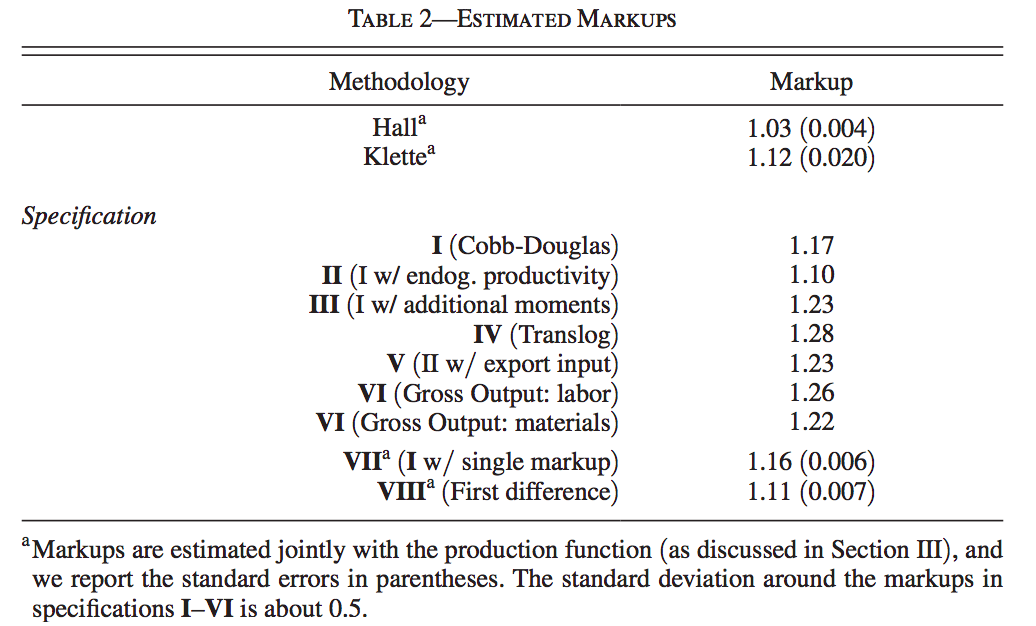
\includegraphics[scale=.35]{DLW-Table2.png}

\end{frame}

\begin{frame}[c]\frametitle{DLW Findings}
    
\centering
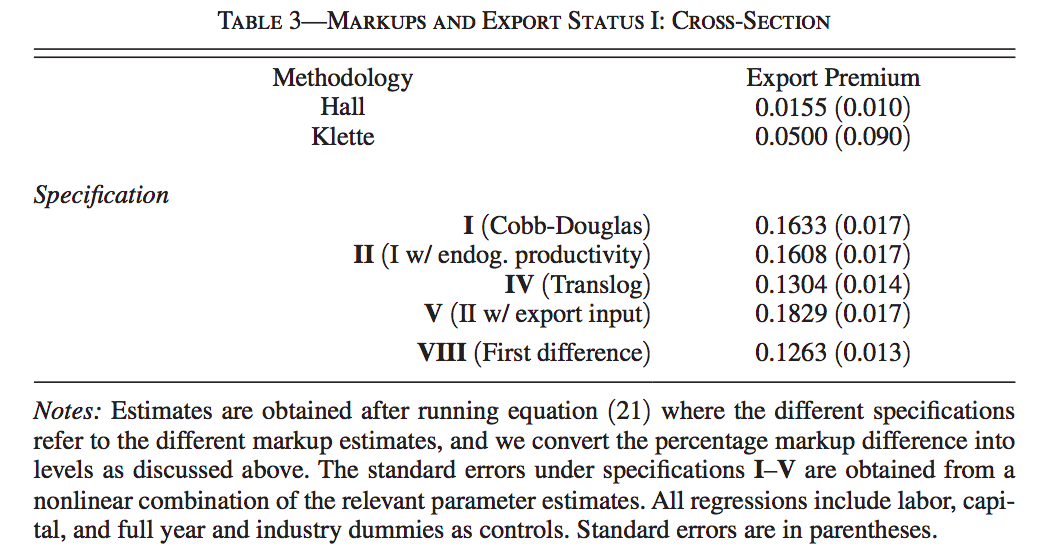
\includegraphics[scale=.4]{DLW-Table3.png}

\end{frame}


\begin{frame}[c]\frametitle{Some Criticisms}
\framesubtitle{That we won't have too much time for...and there are numerous}

\begin{wideitemize}
	\item C-D, trans-log, Hicks-neutral productivity
	\begin{wideitemize}
		\item The ``demand estimation'' literature has spent a lot of effort making their methodology flexible.
	\end{wideitemize}
	\item Relatedly, DLW sell their paper as estimating markups without ``specifying how firms compete in the product market.''
	\begin{wideitemize}
		\item For different levels of concentrations should we expect different $m()$?
		\item Concentration variable in $\mathbf{z}$?
		\item More generally should markups affect input demand?
		\item Have data only on revenues rears its ugly head too b/c firms are not price takers...
		$$ \frac{\partial R}{\partial X^v} = \frac{\partial Q}{\partial X^v} (P + \frac{\partial P}{\partial Q}) $$
	\end{wideitemize}
	

\end{wideitemize}   

\end{frame}


\begin{frame}[c]\frametitle{De Loecker, Eckhout, and Unger (2020) I}

\begin{wideitemize}
	\item U.S. markups rise from 21\% to 64\% since 1980. (after being stable)
	\item Use data from Compustat (and Census). 
	\item Address criticism that output prices vary across firms \textbf{because} markups vary. 
	\begin{wideitemize}
		\item Must control for markups in the production function.
		$$q_{it} + p_{it} = \theta_c \tilde{v}_it + \theta_k \tilde{k}_it + ln(\mu_{it}) + \varepsilon_{it}$$		
	\end{wideitemize}
	\item They point out that market shares determine market power. [what do you think?]
	\item Use market shares as a second proxy variable.
\end{wideitemize}
    
\end{frame}


\begin{frame}[c]\frametitle{De Loecker, Eckhout, and Unger (2020) II}
	\begin{wideitemize}
	       	\item Use ``Cost of Goods Sold'' as variable input. 
	       	\item What is this? 
	       	\begin{wideitemize}
	       	 	\item Is everything in here variable?
	       	 	\item Has the definition changed over time?
	       	 \end{wideitemize}	 
	       	 \item What economic object(s) do these accounting measures captures.	       	       	
	\end{wideitemize}	                      
\end{frame}    


\begin{frame}[c]\frametitle{Markups Over Time}
    \centering
    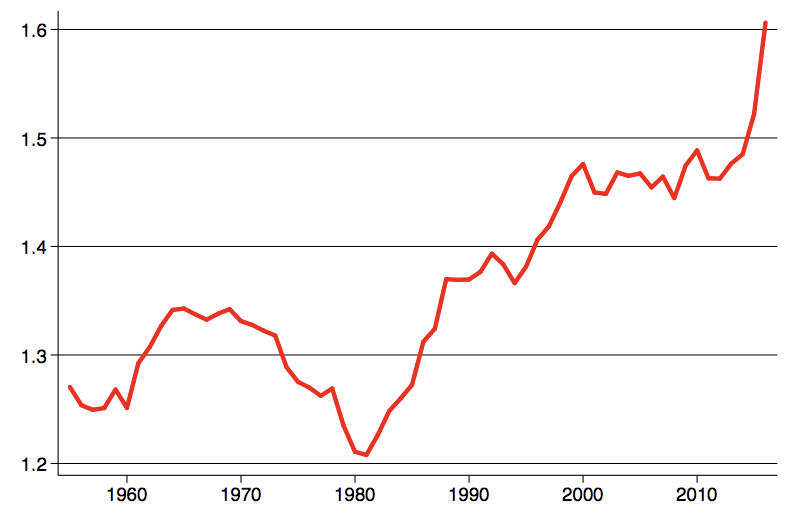
\includegraphics[scale=.7]{DLE1.png}


\end{frame}

\begin{frame}[c]\frametitle{Markups Over Time}
    \centering
    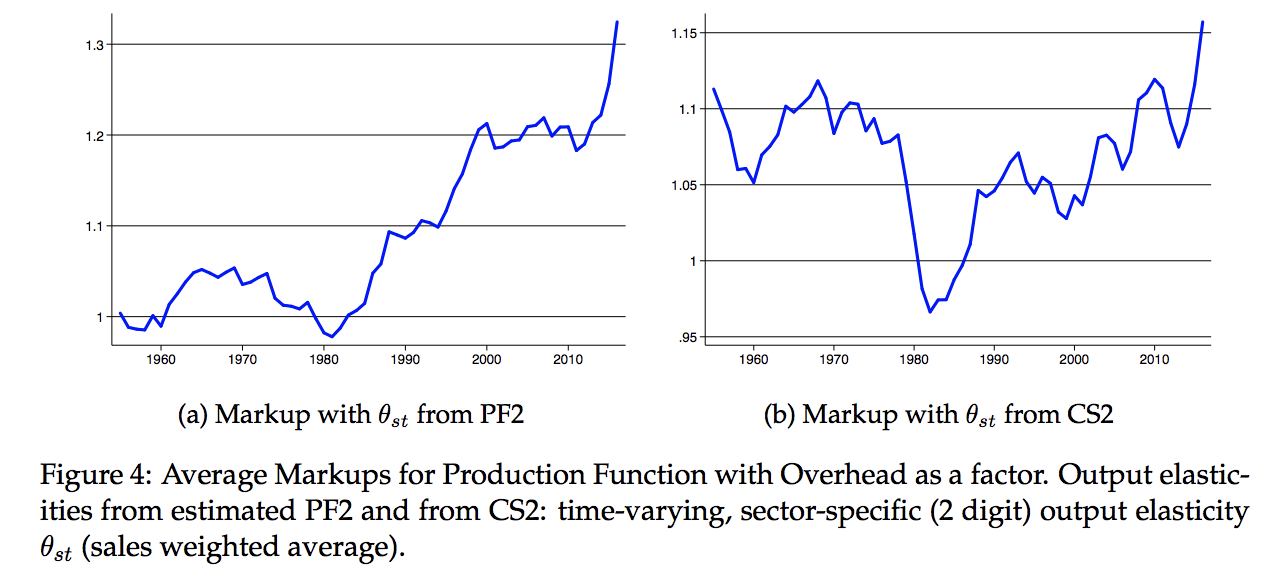
\includegraphics[scale=.7]{DLE4.png}

\end{frame}

\begin{frame}[c]\frametitle{Distribution Markups Over Time}
    \centering
    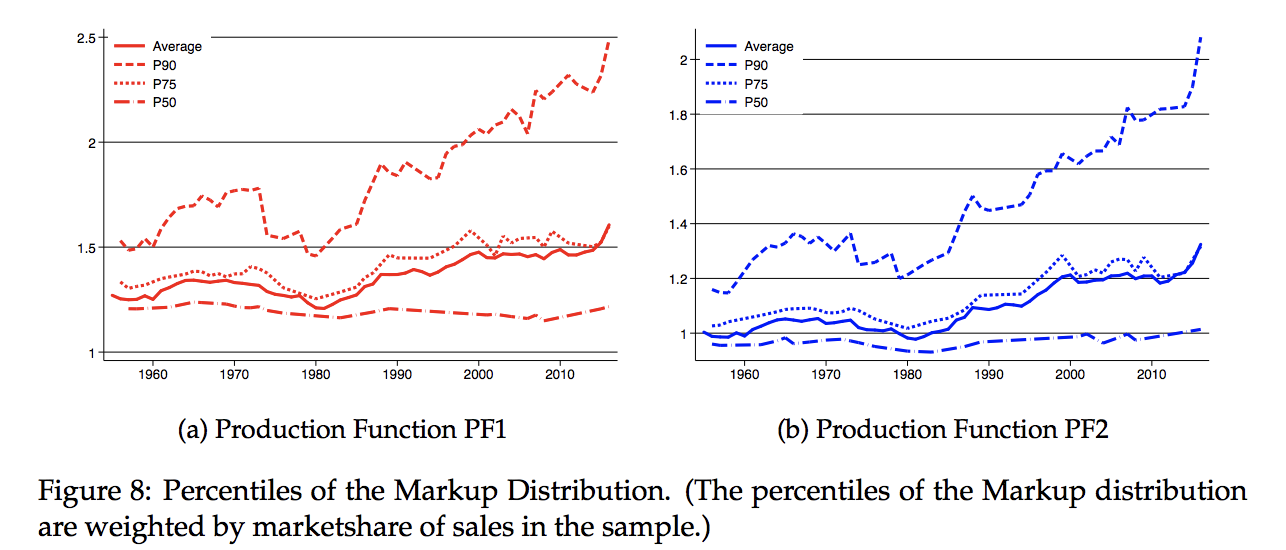
\includegraphics[scale=.7]{DLE8.png}

\end{frame}

\begin{frame}[c]\frametitle{Markups Over Time by Sector}
    \centering
    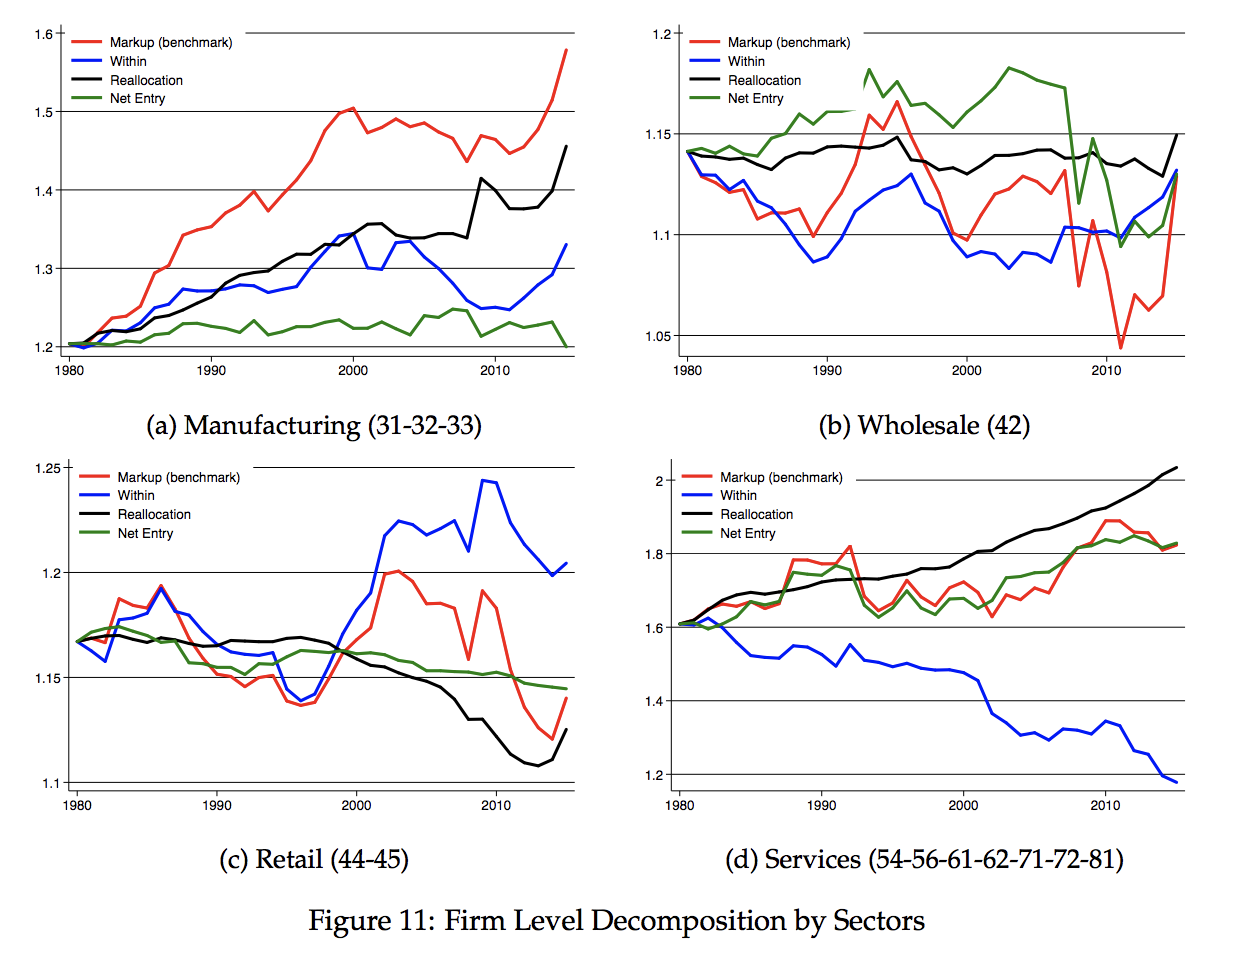
\includegraphics[scale=.5]{DLE11.png}

\end{frame}

\begin{frame}[c]\frametitle{Traina (2018)}
    \begin{wideitemize}
    	\item Difference from DLEG -- variable costs include SG\&A.
    \end{wideitemize}
    
    \centering
    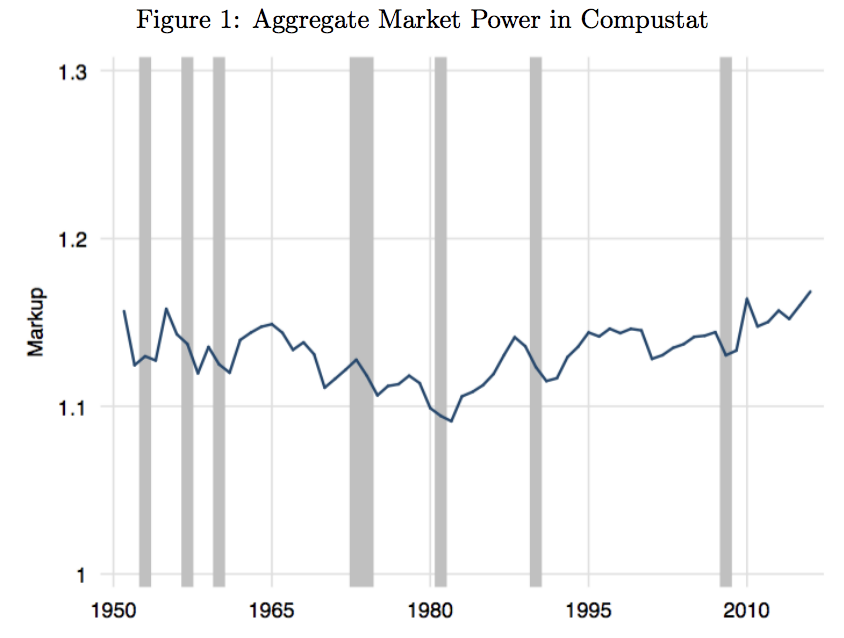
\includegraphics[scale=.6]{Traina1.png}


\end{frame}

\begin{frame}[c]\frametitle{Traina (2018)}
    \begin{wideitemize}
    	\item ``...correctly measuring variable costs is vitally important to getting the facts about markups right.''
    	\item ``...a significant part of the original markup estimation is misattribution of markups to SGA variable costs.''
    \end{wideitemize}
    
    \centering
    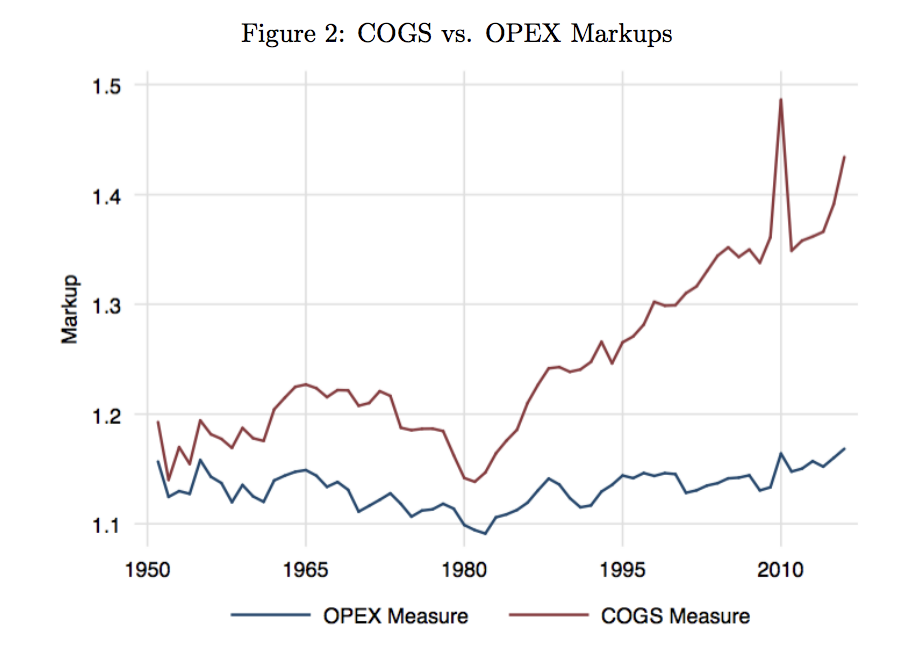
\includegraphics[scale=.55]{Traina2.png}


\end{frame}


\begin{frame}[c]\frametitle{Raval (2019)}
    
\begin{wideitemize}
	\item Which input variable should we use?
	\item Which production function should we use?
\end{wideitemize}

\centering
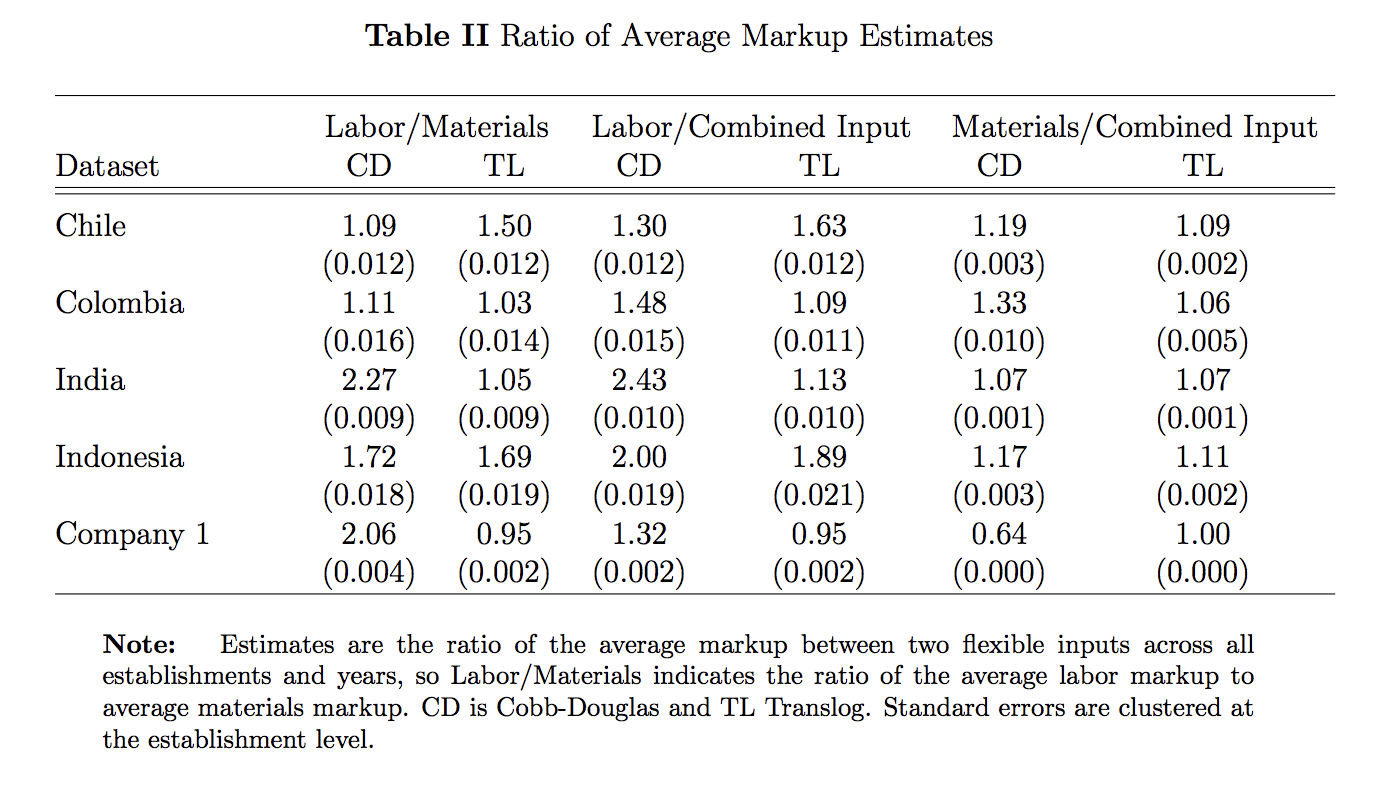
\includegraphics[scale=.45]{RavalT2.png}

\end{frame}




\begin{frame}[c]\frametitle{Bond, Hashemi, Kaplan, Zoch (working paper)}
\framesubtitle{Some Unpleasant Markup Arithmatic: Production Function Elasticities and their
Estimation from Production Data}    

\Skip
1. \textbf{Identification}
Ratio estimator using revenue elasticity, in place of output elasticity, contains
no information about markups.

\Skip\Skip\Skip
2. \textbf{Estimation}\\
It is not possible to estimate output elasticities using revenue data if firms have
market power in output markets.

\end{frame}


\begin{frame}[c]\frametitle{Identification}
    
If firms have output market power, FOC w.r.t. Q in cost minimization:

\[
	\frac{P}{C'(Q)} = \frac{\epsilon_{Q,P}}{\epsilon_{Q,P} - 1}
\]

\Skip\Skip
Why? As you produce more you march down the demand curve.

\begin{align*}
	\hat{\mu_R} &= \frac{\epsilon_{Q,P} - 1}{\epsilon_{Q,P}} \hat{\mu}_Q \\
	&= \frac{C'(Q)}{P} \frac{P}{C'(Q)}
\end{align*}


\end{frame}


\begin{frame}[c]\frametitle{Estimation}

\[    
 r_{it} = \beta_{K} k_{it} + \beta_{L}\ell_{it} + \beta_{M} m_{it} + 
 \omega_{it} + \textcolor{red}{p_{it}} + \epsilon_{it}   
\]

because $r_{it} = y_{it} - \textcolor{red}{p_{it}}$

\Skip
\textbf{Takeaway}: Identifying $\beta_M$ using revenue data would require an instrument
that: (i) shifts demand for $m_{it}$; and (ii) is orthogonal to $p_{it}$.

\Skip\Skip
(Screenshot from authors slide-deck.)
\Skip
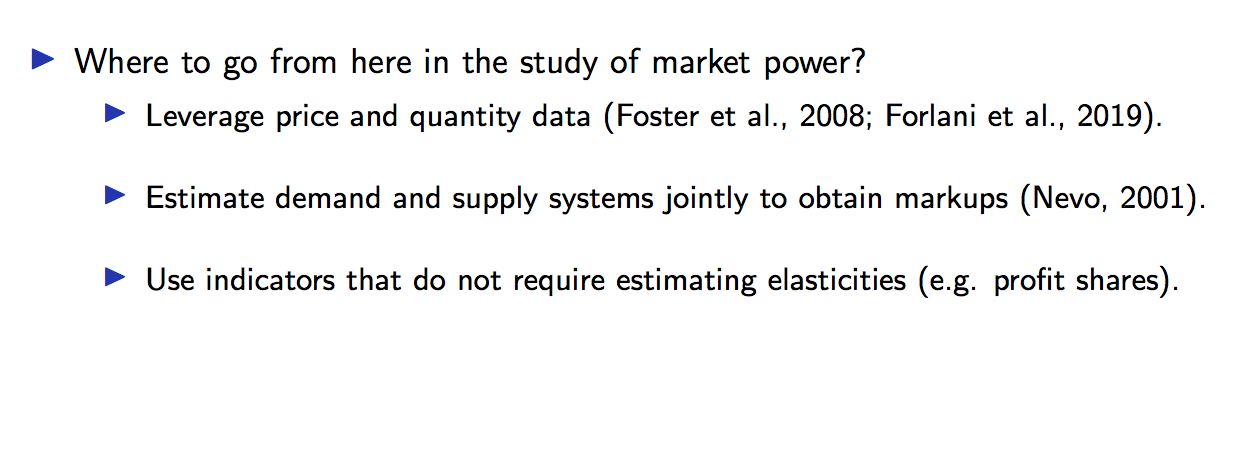
\includegraphics[height=0.45\textheight]{BondScreenshot.png}

\end{frame}


% section de_loecker_and_warzynski_ (end)



\end{document}